\section{TimeBench: Một mô hình dữ liệu và thư viện hỗ trợ cho việc phân tích trực quan hóa dữ liệu chuỗi thời gian}
Dữ liệu chuỗi thời gian đóng một vai trò quan trọng trong nhiều trường hợp cần phân tích hình ảnh và trực quan hóa, chẳng hạn như khi tìm kiếm những thông tin giá trị từ bộ dữ liệu hồ sơ sức khỏe điện tử hoặc xác định các vấn đề mới phát sinh và các kết nối dễ bị hư hại trong mạng truyền thông. Tuy nhiên, nhiều thư viện phần mềm hỗ trợ phân tích trực quan hiện nay chỉ coi thời gian là một loại dữ liệu số phẳng và vì thế đã giải quyết không triệt để sự phức tạp của miền thời gian, chẳng hạn như độ chi tiết của biểu lịch và các khoảng thời gian. Do đó, các nhà phát triển công cụ, kỹ thuật trực quan hóa nâng cao phải triển khai lặp đi lặp lại các nền tảng liên quan đến thời gian trong bộ mã của họ.
TimeBench [339] là một phần mềm mã nguồn mở và miễn phí cung cấp các cấu trúc dữ liệu nền tảng và thuật toán phục vụ cho việc phân tích và trực quan hóa dữ liệu chuỗi thời gian (http://timebench.org). Khả năng biểu đạt thông tin và khả năng dễ dàng tiếp cận của nó đã được đánh giá thông qua nhiều ứng dụng cụ thể khi giải quyết các thách thức liên quan đến dữ liệu chuỗi thời gian và các nghiên cứu phát triển dài hạn được ở cả cấp độ các chương trình nghiên cứu lẫn các dự án của sinh viên. Hình (\ref{fig:f7.16}) thể hiện 7 ứng dụng khác nhau được phát triển với thư viện TimeBench.
\begin{figure}[H] % places figure environment here   
    \centering % Centers Graphic
    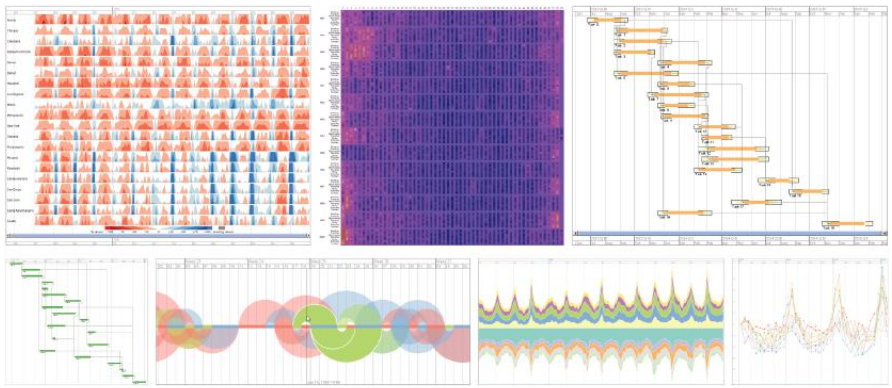
\includegraphics[width=1\textwidth]{assets/fig_7_16.png} 
    \caption{TimeBench [339]. Ví dụ về các ứng dụng được xây dựng dựa trên TimeBench: (1) Dữ liệu sức khỏe hàng tháng của 20 thành phố trong 14 năm trong biểu đồ miền [331]; (2) Dữ liệu sức khỏe hàng ngày trong khoảng thời gian 14 năm được thể hiện trong một biểu đồ GROOVE [262]; (3) Bản kế hoạch dự án sử dụng PlanningLines [4]; (4) Bản kế hoạch dự án dưới dạng biểu đồ Gantt [170]; (5) Sơ đồ vòng cung [451] thể hiện mối quan hệ giữa ba loại sự kiện; (6) Trực quan hóa ThemeRiver [172]; (7) Các biểu đồ đường đi kèm chỉ mục [34]. Dữ liệu sức khỏe từ nghiên cứu NMMAPS [316] được sử dụng trong (1), (2), (5), (6) và (7). (http://timebench.org).} % Creates caption underneath graph
    \label{fig:f7.16}
\end{figure}